\chapter{Verification and application examples}
\label{cha:examples}

This chapter validates the implementation against closed-form solutions,
quantifies the accuracy of the contact model in a controlled single-collision
experiment, and finally applies the model to the full deposition--compression
problem of Section~\ref{sec:problem}.  Every number reported here was produced
with the code in this repository; the commands needed to reproduce them are
given with each example.

\section{Unit verification against closed-form results}
\label{sec:unit-tests}

The automated test suite is executed with
\begin{verbatim}
  python -m pytest tests/ -q
\end{verbatim}
and contains \num{101} tests, grouped by module, which include checks that
invalid input is rejected with a specific message.  The four examples below each
isolate one equation of Chapter~\ref{cha:formulation}.  Further tests compare
complete simulations with closed-form results: the static Hertz overlap of a
particle resting on a wall, a single contact for a particle on or next to a
vertex shared by two edges, conservation of momentum in an oblique collision,
the equilibrium of a strip footing and of a platen on a side wall, the removal
of particles through an open edge, and the filling of a trapezoidal domain.  All
tests pass.

\subsection{Example 1 -- free fall of a single body}

\paragraph{Purpose.}  Verify the velocity-Verlet
implementation~\eqref{eq:vv1}--\eqref{eq:vv4}.

\paragraph{Setup.}  One body, no contacts, constant acceleration
$\mathbf{a}=-g\,\mathbf{e}_{y}$ with $g=\qty{9.81}{\metre\per\second\squared}$,
starting from rest at the origin, one step of
$\Delta t=\qty{1e-3}{\second}$.

\paragraph{Reference solution.}  For a constant acceleration the scheme is not
merely second-order accurate but \emph{exact}, because the Taylor expansion of
the trajectory truncates:
\begin{equation}
  y(\Delta t) = -\tfrac{1}{2}g\,\Delta t^{2},
  \qquad
  v_{y}(\Delta t) = -g\,\Delta t .
\end{equation}

\paragraph{Result.}  The computed values reproduce
$y=\qty{-4.905e-6}{\metre}$ and $v_{y}=\qty{-9.81e-3}{\metre\per\second}$ to
machine precision, which confirms both the ordering of the kick--drift--kick
stages and the absence of a spurious $\Delta t$ factor.

\subsection{Example 2 -- Hertzian normal force}

\paragraph{Purpose.}  Verify the elastic branch~\eqref{eq:hertz} of the normal
law together with the effective quantities~\eqref{eq:effective}.

\paragraph{Setup.}  Two equal particles, $R=\qty{10}{\milli\metre}$, overlap
$\delta_{n}=\qty{0.1}{\milli\metre}$, zero relative velocity (so that the
dashpot is inactive), and $e=1$ so that $\beta=0$.  The effective radius is
$R^{*}=R/2=\qty{5}{\milli\metre}$.

\paragraph{Reference solution.}
\begin{equation}
  k_{n} = \tfrac{4}{3}E^{*}\sqrt{R^{*}}
        = \tfrac{4}{3}\,(\qty{2.6667e6}{\pascal})\sqrt{\qty{5e-3}{\metre}}
        = \qty{2.5142e5}{\newton\per\metre^{3/2}},
\end{equation}
\begin{equation}
  F_{n} = k_{n}\,\delta_{n}^{3/2}
        = \qty{2.5142e5}{} \times (\qty{1e-4}{})^{3/2}
        = \qty{0.251416}{\newton} .
\end{equation}

\paragraph{Result.}  The model returns $F_{x}=\qty{0.2514157}{\newton}$, in
agreement to a relative tolerance of $10^{-12}$, with $F_{y}$ and both
tangential components identically zero -- confirming that a purely normal
approach generates no shear.

\subsection{Example 3 -- Coulomb sliding limit}

\paragraph{Purpose.}  Verify the return mapping~\eqref{eq:coulomb}.

\paragraph{Setup.}  The same contact as in Example 2, with $\mu=0.5$ and a
large tangential relative velocity $v_{t}=\qty{5}{\metre\per\second}$ imposed
over $\Delta t=\qty{1e-5}{\second}$.  The tangential stiffness is
$S_{t}=8G^{*}\sqrt{R^{*}\delta_{n}}=\qty{3232.5}{\newton\per\metre}$ and the
spring accumulated in one step is
$\lVert\boldsymbol{\xi}\rVert=v_{t}\Delta t=\qty{5e-5}{\metre}$, so the trial
spring force alone,
$S_{t}\lVert\boldsymbol{\xi}\rVert=\qty{0.162}{\newton}$, already exceeds the
friction cone.

\paragraph{Reference solution.}
\begin{equation}
  \lVert\mathbf{F}_{t}\rVert = \mu F_{n}
  = 0.5\times\qty{0.251416}{\newton} = \qty{0.125708}{\newton}.
\end{equation}

\paragraph{Result.}  The returned tangential force equals $\mu F_{n}$ to within
a relative tolerance of $10^{-9}$, and never exceeds it.  This confirms both the
scaling of the force onto the cone and the consistency of the spring reset
$\boldsymbol{\xi}=-\mathbf{F}_{t}/S_{t}$.

\subsection{Example 4 -- effective moduli}

\paragraph{Purpose.}  Verify~\eqref{eq:moduli}.

\paragraph{Reference solution.}  For $E=\qty{5}{\mega\pascal}$ and $\nu=0.25$:
$G=E/[2(1+\nu)]=\qty{2.0}{\mega\pascal}$,
$E^{*}=E/[2(1-\nu^{2})]=\qty{2.6667}{\mega\pascal}$ and
$G^{*}=G/[2(2-\nu)]=\qty{0.57143}{\mega\pascal}$.

\paragraph{Result.}  All three constants match, and both effective moduli are
positive, which guards against a sign error in the $(1-\nu^{2})$ or $(2-\nu)$
factors.

\section{Component test: binary collision and restitution}
\label{sec:component-tests}

\subsection{Set-up}

The four unit tests above check individual expressions but not the dynamic
behaviour that emerges from their combination.  The classical benchmark for a
soft-sphere contact model is the head-on collision of two identical grains: the
model should return exactly the restitution coefficient $e$ that was prescribed
as an input, and that value should be independent of the impact velocity.

Two particles of radius $R=\qty{10}{\milli\metre}$ of the reference material are
launched against each other with relative velocity $v_{\text{rel}}=2v_{0}$ and
integrated with the same velocity-Verlet scheme until they separate.  The
measured restitution is
\begin{equation}
  e_{\text{out}}
  = \frac{\lvert v_{\text{rel}}^{\,\text{after}}\rvert}
         {\lvert v_{\text{rel}}^{\,\text{before}}\rvert}.
\end{equation}
A very small time step ($\alpha=0.02$, i.e.\ $\Delta t=T_{R}/50$) is used so
that the integration error is negligible and only the \emph{constitutive} error
is measured.

\subsection{Results}

\begin{table}[htbp]
  \centering
  \caption{Restitution reproduced by the Hertz--Tsuji contact model,
  $R=\qty{10}{\milli\metre}$, $\Delta t = 0.02\,T_{R}$.}
  \label{tab:restitution}
  \begin{tabular}{S[table-format=1.2]S[table-format=1.2]S[table-format=1.4]S[table-format=2.2]S[table-format=1.4]S[table-format=3.0]}
    \toprule
    {$e$ (input)} & {$v_{\text{rel}}$ [\unit{\metre\per\second}]} &
    {$e_{\text{out}}$} & {error [\%]} &
    {$t_{c}$ [\unit{\milli\second}]} & {steps} \\
    \midrule
    0.90 & 0.50 & 0.9022 &  0.25 & 3.172 & 131 \\
    0.90 & 1.00 & 0.9022 &  0.25 & 2.761 & 114 \\
    0.70 & 0.50 & 0.7185 &  2.64 & 3.269 & 135 \\
    0.70 & 1.00 & 0.7186 &  2.66 & 2.833 & 117 \\
    0.50 & 0.50 & 0.5505 & 10.10 & 3.390 & 140 \\
    0.50 & 1.00 & 0.5505 & 10.11 & 2.954 & 122 \\
    0.40 & 0.50 & 0.4721 & 18.02 & 3.487 & 144 \\
    0.40 & 1.00 & 0.4721 & 18.03 & 3.051 & 126 \\
    0.20 & 0.50 & 0.3246 & 62.29 & 3.802 & 157 \\
    0.20 & 1.00 & 0.3246 & 62.29 & 3.293 & 136 \\
    \bottomrule
  \end{tabular}
\end{table}

Table~\ref{tab:restitution} supports three conclusions.

\begin{enumerate}[leftmargin=2.2em]
  \item \textbf{Velocity independence is excellent.}  Doubling the impact
        velocity changes $e_{\text{out}}$ by less than $0.02\%$.  This is the
        property that the Tsuji scaling $c_{n}\propto\sqrt{S_{n}m^{*}}$ was
        designed to deliver, and it is reproduced essentially exactly.  A model
        with a constant (velocity-independent) dashpot would show a strong
        drift here.
  \item \textbf{There is a systematic positive bias in $e$.}  The measured
        restitution always exceeds the prescribed one, and the discrepancy grows
        rapidly as $e$ decreases: negligible at $e=0.9$, $10\%$ at $e=0.5$, and
        $62\%$ at $e=0.2$.  The cause is well known and is not an implementation
        error: relation~\eqref{eq:beta} is the exact solution for a
        \emph{linear} spring--dashpot oscillator, whereas the contact here is
        Hertzian, with a stiffness that vanishes at the beginning and at the end
        of the collision.  The dashpot is therefore weak exactly where the
        linear theory assumes it to be strong, and less energy is
        dissipated~\cite{direnzo2004,thornton2013}.
  \item \textbf{Practical consequence.}  The input $e$ should be regarded as a
        \emph{damping parameter}, not as a directly measurable restitution
        coefficient.  If a specific restitution must be reproduced,
        Table~\ref{tab:restitution} can be read backwards: to obtain a physical
        $e\approx0.4$ one should prescribe $e\approx0.28$.  The reference
        simulation uses $e=0.4$ as an input, which corresponds to an effective
        restitution of about $0.47$.
\end{enumerate}

\subsection{Time-step convergence}

The same experiment, repeated at $e=0.4$ and
$v_{\text{rel}}=\qty{0.5}{\metre\per\second}$ with a decreasing time step,
isolates the \emph{integration} error from the constitutive error.

\begin{table}[htbp]
  \centering
  \caption{Convergence of the measured restitution with the time step
  ($e=0.4$, $v_{\text{rel}}=\qty{0.5}{\metre\per\second}$).}
  \label{tab:dt-convergence}
  \begin{tabular}{S[table-format=1.3]S[table-format=1.3e2]S[table-format=3.0]S[table-format=1.4]S[table-format=1.2]}
    \toprule
    {$\alpha=\Delta t/T_{R}$} & {$\Delta t$ [\unit{\second}]} &
    {steps per collision} & {$e_{\text{out}}$} & {error [\%]} \\
    \midrule
    0.200 & 2.422e-4 &  14 & 0.4817 & 2.05 \\
    0.100 & 1.211e-4 &  29 & 0.4744 & 0.51 \\
    0.050 & 6.054e-5 &  58 & 0.4729 & 0.19 \\
    0.020 & 2.422e-5 & 144 & 0.4721 & 0.02 \\
    0.010 & 1.211e-5 & 289 & 0.4720 & {--} \\
    \bottomrule
  \end{tabular}
\end{table}

The measured restitution converges monotonically to $0.4720$, and the error
falls by roughly a factor of four when $\Delta t$ is halved, consistent with the
second-order accuracy claimed in Section~\ref{sec:integration}.  At the
production setting $\alpha=0.2$ the integration error is only $2\%$, an order of
magnitude smaller than the constitutive bias discussed above.  This justifies
the choice~\eqref{eq:dt}: refining the time step further would improve the
integration but not the physics.

\section{Reference simulation: deposition and confined compression}
\label{sec:reference-run}

\subsection{Set-up}

The complete experiment is run with
\begin{verbatim}
  python main.py
\end{verbatim}
which writes \texttt{output/simulation.gif} and
\texttt{output/load\_displacement.png}.  The inputs are listed in
Table~\ref{tab:refsetup}.  The top edge of the box is a loaded platen: it
closes the box while it is filled and is seated on the bed when loading starts.

\paragraph{Version of the results.}  The results in the remainder of this
section and in Section~\ref{sec:load-level} were obtained with the first version
of the code, before the corrections described in Sections~\ref{sec:history}
and~\ref{sec:deposition}.  That version biased the packing towards small
particles, as discussed below.  With the current code the box holds \num{179}
particles with a mean radius of \qty{12.25}{\milli\metre}, so a fresh run of
\texttt{main.py} does not reproduce Tables~\ref{tab:packing}
to~\ref{tab:loadhistory} or the figures of these sections, which should be
regenerated before they are quoted.

\begin{table}[htbp]
  \centering
  \caption{Input parameters of the reference simulation.}
  \label{tab:refsetup}
  \begin{tabular}{lll}
    \toprule
    Group & Parameter & Value \\
    \midrule
    Geometry & box width $B$          & \qty{0.20}{\metre} \\
             & box height $L$         & \qty{0.60}{\metre} \\
             & radius range $[R_{\min},R_{\max}]$ & $[4,\ 20]$ \unit{\milli\metre} \\
    \midrule
    Material & density $\rho$         & \qty{2500}{\kilogram\per\cubic\metre} \\
             & Young's modulus $E$    & \qty{5}{\mega\pascal} \\
             & Poisson ratio $\nu$    & 0.25 \\
             & restitution $e$        & 0.40 \\
             & friction $\mu$         & 0.50 \\
    \midrule
    Loading  & platen mass $m_{p}$    & \qty{0.5}{\kilogram} \\
             & peak load $F_{\max}$   & \qty{1000}{\newton} \\
             & ramp duration $t_{r}$  & \qty{0.4}{\second} \\
             & hold after ramp        & yes \\
             & compression duration   & \qty{1.0}{\second} \\
    \midrule
    Numerics & gravity $g$            & \qty{9.81}{\metre\per\second\squared} \\
             & time step $\Delta t$   & \qty{9.686e-5}{\second} \\
             & rest between stages    & \qty{0.1}{\second} \\
             & random seed            & 7 \\
    \bottomrule
  \end{tabular}
\end{table}

\subsection{Deposition stage}

\begin{figure}[htbp]
  \centering
  \begin{subfigure}[b]{0.31\textwidth}
    \centering
    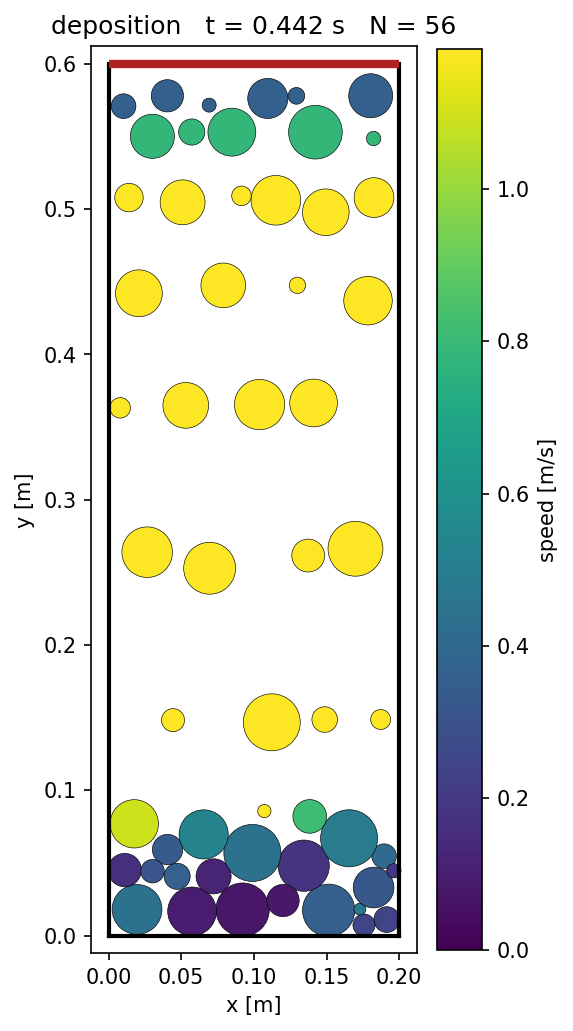
\includegraphics[width=\textwidth]{figures/deposition_early.png}
    \caption{early raining}
  \end{subfigure}
  \hfill
  \begin{subfigure}[b]{0.31\textwidth}
    \centering
    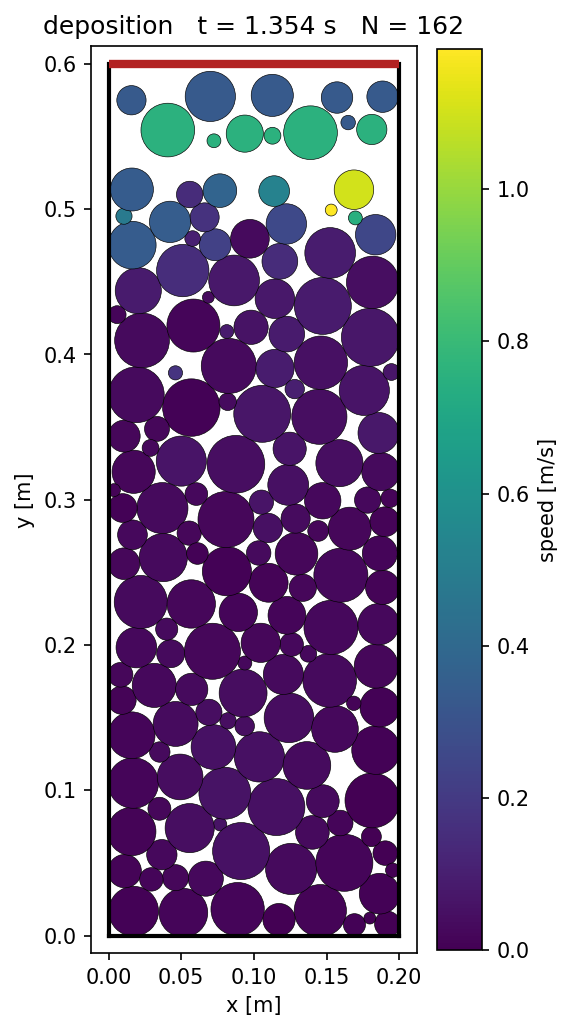
\includegraphics[width=\textwidth]{figures/deposition_mid.png}
    \caption{bed nearly complete}
  \end{subfigure}
  \hfill
  \begin{subfigure}[b]{0.31\textwidth}
    \centering
    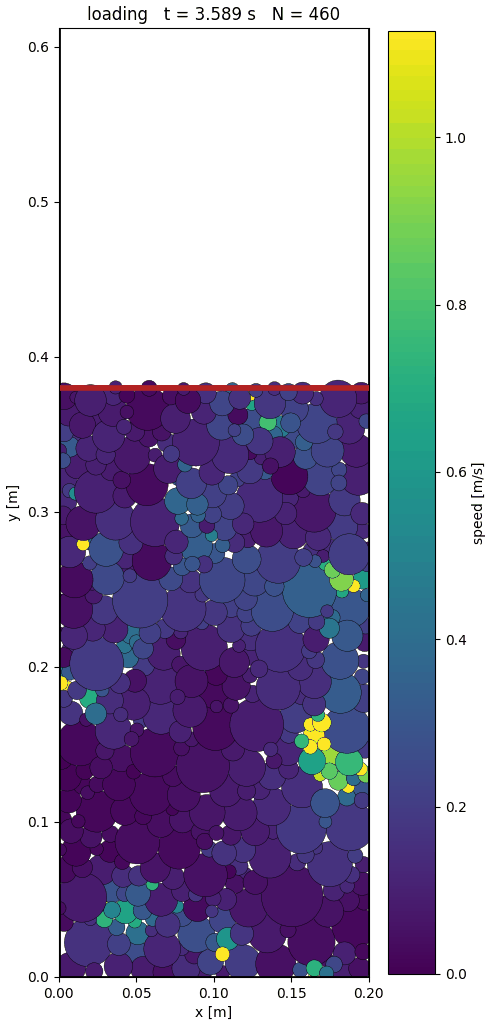
\includegraphics[width=\textwidth]{figures/loading_final.png}
    \caption{end of loading}
  \end{subfigure}
  \caption{Snapshots of the reference simulation, coloured by particle speed.
  Waves of particles are inserted near the top and rain down (a, b) until the
  bed reaches the insertion band; the platen (red line) then compresses the
  packing (c).  Note the deep interpenetration visible in (c), which is
  discussed in Section~\ref{sec:load-level}.}
  \label{fig:snapshots}
\end{figure}

Raining terminates by itself after \num{460} particles, when the bed reaches the
insertion band.  The state at the end of the settling phase is summarised in
Table~\ref{tab:packing}.

\begin{table}[htbp]
  \centering
  \caption{Properties of the deposited packing (after settling, before loading).}
  \label{tab:packing}
  \begin{tabular}{lll}
    \toprule
    Quantity & Value & Comment \\
    \midrule
    Number of particles $N$          & 460 & determined by the geometry \\
    Bed height                       & \qty{0.5835}{\metre} & \num{97}\% of $L$ \\
    Mean radius $\bar{R}$            & \qty{7.6}{\milli\metre} & input range $[4,20]$ \unit{\milli\metre} \\
    Standard deviation of $R$        & \qty{3.2}{\milli\metre} & \\
    Area fraction $\phi$             & 0.840 & dense random packing \\
    Particle--particle contacts      & 843  & \\
    Coordination number $Z$          & 3.67 & \\
    Mean overlap $\delta_{n}/R$      & \num{3.6}\% & under self-weight only \\
    Maximum overlap $\delta_{n}/R$   & \num{21.0}\% & deepest contact \\
    Mean kinetic energy $\bar{E}_{k}$& \qty{1.3e-9}{\joule} & quiescence
                                       tolerance \qty{1e-6}{\joule} \\
    \bottomrule
  \end{tabular}
\end{table}

Three observations deserve comment.

\paragraph{The realised size distribution is not uniform.}  Although radii are
drawn from $\mathcal{U}(\qty{4}{\milli\metre},\qty{20}{\milli\metre})$, whose
mean is \qty{12}{\milli\metre}, the mean radius of the deposited assembly is
only \qty{7.6}{\milli\metre}, and the histogram decreases monotonically with
size (\num{192} particles below \qty{6}{\milli\metre} against a single one above
\qty{18}{\milli\metre}).  The reason is the rejection sampling of
Section~\ref{sec:deposition}: a large candidate is far more likely to overlap an
existing grain and to exhaust its \num{30} placement attempts, so the acceptance
probability decreases sharply with $R$.  The insertion procedure therefore
biases the distribution.  The current code removes this bias by drawing each
radius once and retrying it, largest first, until it is placed
(Section~\ref{sec:deposition}).

\paragraph{The packing is dense and well connected.}  An area fraction of
\num{0.840} and a coordination number of \num{3.67} are typical of a
polydisperse two-dimensional random close packing.  A value of $Z$ above the
isostatic threshold for frictional discs ($Z=3$) confirms that the assembly is
mechanically stable rather than marginally rigid.

\paragraph{The overlaps are already large under self-weight.}  A mean
$\delta_{n}/R$ of \num{3.6}\% before any external load is applied is well above
the one per cent guideline of~\eqref{eq:overlap-criterion}.  It is a direct
consequence of the artificial softening: the estimate~\eqref{eq:delta-static}
with a contact force of about \qty{1}{\newton} -- the weight of the column
carried by a bottom contact -- and $R^{*}=\bar{R}/2$ gives
$\delta_{n}=\qty{0.27}{\milli\metre}$, i.e.\ \num{3.6}\% of $\bar{R}$, in exact
agreement with the measurement.  The deposited packing should therefore be
regarded as qualitatively, not quantitatively, representative; raising $E$ is
the remedy.

\subsection{Compression stage}

\begin{figure}[htbp]
  \centering
  \includegraphics[width=\textwidth]{../output/load_displacement.png}
  \caption{Reference simulation, $F_{\max}=\qty{1000}{\newton}$.  Left: applied
  load $F(t)$ and contact reaction $F_{p}$ against loading time.  Right:
  reaction against platen displacement.}
  \label{fig:loadcurve1000}
\end{figure}

Figure~\ref{fig:loadcurve1000} shows the response.  The applied load ramps
linearly to \qty{1000}{\newton} over \qty{0.4}{\second} and is then held for a
further \qty{0.6}{\second}.  The contact reaction $F_{p}$ tracks $F(t)$ closely
throughout the ramp and settles at \qty{992.7}{\newton} at the end of the hold,
i.e.\ within \num{0.7}\% of the applied value.  This is the system-level
consistency check announced in Section~\ref{sec:verification}: at equilibrium
Eq.~\eqref{eq:platen-eom} requires $F_{p}=F(t)$, and the small residual measures
how far the platen still is from static equilibrium.

The final platen displacement is $u_{p}=\qty{203.8}{\milli\metre}$, i.e.\ a
nominal axial strain of \num{35}\% of the initial bed height.  Such a strain
cannot be produced by grain rearrangement alone in a packing that is already
dense; it is produced by interpenetration.  Consistently with
Table~\ref{tab:overlap}, a load of \qty{1000}{\newton} distributed over the
handful of contacts under the platen implies overlaps of the order of half a
radius, and the snapshot of Figure~\ref{fig:snapshots}(c) shows the grains
visibly merging.  This case is therefore \emph{outside} the validity range of
the Hertz--Mindlin law and is retained here as a deliberate illustration of what
excessive loading looks like.

\section{Effect of the load level}
\label{sec:load-level}

To quantify the previous statement, the identical packing (same seed, same
deposition history) was compressed with a peak load of \qty{100}{\newton}
instead of \qty{1000}{\newton}; the case is reproduced by setting
\texttt{amplitude=100.0} in the \texttt{Heaviside} load of
\texttt{build\_simulation}.  The result is
Figure~\ref{fig:loadcurve100} and Table~\ref{tab:loadlevels}.

\begin{figure}[htbp]
  \centering
  \includegraphics[width=\textwidth]{../output/load_displacement_100N.png}
  \caption{Same packing compressed with $F_{\max}=\qty{100}{\newton}$.  The
  reaction follows the applied ramp with a mean deviation of
  \qty{0.02}{\newton} during the hold, and the load--displacement curve is
  smooth and monotonic.}
  \label{fig:loadcurve100}
\end{figure}

\begin{table}[htbp]
  \centering
  \caption{Response of the same packing at two load levels.}
  \label{tab:loadlevels}
  \begin{tabular}{lS[table-format=3.1]S[table-format=3.1]}
    \toprule
    Quantity & {$F_{\max}=\qty{100}{\newton}$} & {$F_{\max}=\qty{1000}{\newton}$} \\
    \midrule
    Final platen displacement $u_{p}$ [\unit{\milli\metre}] & 34.3 & 203.8 \\
    Nominal axial strain $u_{p}/h_{0}$ [\%]                 &  5.9 &  34.9 \\
    Final reaction $F_{p}$ [\unit{\newton}]                 & 100.2 & 992.7 \\
    Deviation from the applied load [\%]                    &  0.2 &   0.7 \\
    Estimated $\delta_{n}/\bar{R}$ under the platen [\%]    & 10.6 &  49.2 \\
    Secant stiffness $F_{\max}/u_{p}$ [\unit{\newton\per\milli\metre}] & 2.91 & 4.91 \\
    \bottomrule
  \end{tabular}
\end{table}

A tenfold increase of the load produces only a \num{5.9}-fold increase of the
displacement, so the packing stiffens as it is compressed.  Qualitatively this
is the expected signature of a Hertzian assembly: from~\eqref{eq:hertz} a single
contact obeys $F\propto\delta^{3/2}$, hence a secant stiffness scaling as
$F^{1/3}$, i.e.\ a factor $10^{1/3}=\num{2.15}$ between the two load levels.
The measured ratio is smaller, $4.91/2.91=\num{1.69}$: the assembly is
\emph{softer} than the elastic scaling predicts.  Two effects contribute, both
of them consequences of overloading -- irreversible rearrangement of the
contact network, which adds displacement that no elastic law accounts for, and
the departure of the deeply interpenetrating contacts from the small-overlap
regime in which~\eqref{eq:hertz} was derived.  The comparison is therefore not a
validation of the Hertz exponent but a further indication that the
\qty{1000}{\newton} case is over-loaded.

The detailed history of the \qty{100}{\newton} case is reproduced in
Table~\ref{tab:loadhistory}.  The reaction lags the applied load by less than
\qty{1}{\newton} throughout the ramp, and during the hold it averages
$\qty{100.02}{\newton}$ with a standard deviation of only
$\qty{0.45}{\newton}$ -- a fluctuation of \num{0.45}\%.  The loading is
therefore quasi-static in the sense that inertial effects are negligible, which
is precisely the regime in which an oedometric test should be interpreted.

\begin{table}[htbp]
  \centering
  \caption{Load history for $F_{\max}=\qty{100}{\newton}$.  The ramp ends at
  $t=\qty{0.4}{\second}$.}
  \label{tab:loadhistory}
  \begin{tabular}{S[table-format=1.3]S[table-format=3.2]S[table-format=2.3]S[table-format=3.2]}
    \toprule
    {$t$ [\unit{\second}]} & {$F(t)$ [\unit{\newton}]} &
    {$u_{p}$ [\unit{\milli\metre}]} & {$F_{p}$ [\unit{\newton}]} \\
    \midrule
    0.099 &  24.72 & 12.207 &  25.75 \\
    0.198 &  49.42 & 18.346 &  48.91 \\
    0.302 &  75.58 & 26.214 &  74.97 \\
    0.401 & 100.00 & 34.286 & 101.25 \\
    0.599 & 100.00 & 34.311 &  99.93 \\
    0.802 & 100.00 & 34.359 & 100.30 \\
    1.000 & 100.00 & 34.348 & 100.21 \\
    \bottomrule
  \end{tabular}
\end{table}

The shape of the curve is also informative.  The first \qty{12}{\milli\metre} of
displacement are produced by only a quarter of the load: the platen is placed in
contact with the highest grain of an irregular surface and must first seat
itself on a sufficient number of contacts.  Once the contact network under the
platen is established the response becomes much stiffer and almost linear, with
small load drops that correspond to local rearrangements -- the discrete
analogue of the yielding events observed in real granular assemblies.

\section{Strip footing in a trapezoidal container}
\label{sec:footing}

The script \texttt{examples/footing\_on\_trapezoid.py} exercises the general
input: a non-rectangular domain, a different boundary condition on the edges, a
load applied to part of a side only, and a choice of load histories.  The
container is the trapezoid with vertices $(0.05,0)$, $(0.35,0)$, $(0.40,0.25)$
and $(0,0.25)$~\unit{\metre}, which widens upwards.  Its bottom and left side
are rough walls and its right side is a smooth wall ($\mu_{w}=0$).  The top side
is split into three collinear edges: the outer two are open, and the middle one,
\qty{0.1}{\metre} wide, is a loaded platen of mass \qty{0.3}{\kilogram} that acts
as a rigid strip footing.
\begin{verbatim}
  vertices = [(0.05, 0.0), (0.35, 0.0), (0.40, 0.25),
              (0.25, 0.25), (0.15, 0.25), (0.00, 0.25)]
  boundary_conditions = [Wall(), Wall(friction=0.0), Open(),
                         LoadedPlaten(load=load, mass=0.3), Open(), Wall()]
  geometry = Geometry(vertices, boundary_conditions)
\end{verbatim}
The container is rained full with radii in $[4,8]$~\unit{\milli\metre} up to an
insertion band at $y\in[0.19,0.20]$~\unit{\metre}, which gives \num{482}
particles and leaves about \qty{5}{\centi\metre} of freeboard; the footing is
seated on the fill when loading starts.  A command-line argument selects one of
four load histories -- a pulse, a Heaviside step, a sinusoid, or a time history
that loads, partly unloads and reloads -- with peaks of \qtyrange{5}{6}{\newton}.

These levels were chosen after loading the footing with a slow ramp to
\qty{20}{\newton} over \qty{2}{\second} (Table~\ref{tab:footing}).  The response
stiffens up to about \qty{8}{\newton}, at a settlement of
\qty{10}{\milli\metre}.  Between \qty{10}{\newton} and \qty{12}{\newton} the
settlement jumps from \qty{20}{\milli\metre} to \qty{76}{\milli\metre}, and the
footing punches into the fill while material flows around its ends and over it.
The bearing capacity is therefore about \qty{10}{\newton}, and the example loads
stay at about half of it.  A capacity this low is expected from soft, frictional
discs without rolling resistance (Section~\ref{sec:limitations}).

\begin{table}[htbp]
  \centering
  \caption{Settlement of the strip footing under a slow ramp to
  \qty{20}{\newton} over \qty{2}{\second}.}
  \label{tab:footing}
  \begin{tabular}{S[table-format=2.0]S[table-format=3.2]}
    \toprule
    {$F$ [\unit{\newton}]} & {$u_{p}$ [\unit{\milli\metre}]} \\
    \midrule
     1 &   2.26 \\
     2 &   3.94 \\
     4 &   6.52 \\
     6 &   8.21 \\
     8 &   9.74 \\
    10 &  19.66 \\
    12 &  75.80 \\
    14 & 108.11 \\
    16 & 126.39 \\
    \bottomrule
  \end{tabular}
\end{table}

\section{Suggested further studies}
\label{sec:further}

The examples above exercise every part of the code, but a number of studies are
natural next steps and are directly supported by the existing interfaces.

\begin{enumerate}[leftmargin=2.2em]
  \item \textbf{Softening convergence.}  Repeat the \qty{100}{\newton} case with
        $E=5$, $50$ and \qty{500}{\mega\pascal}.  The time step falls as
        $E^{-1/2}$ and the overlaps as $E^{-2/3}$; the load--displacement curve
        should converge once the overlaps drop below one per cent.  This is the
        single most important study before any quantitative use of the model.
  \item \textbf{Time-step refinement.}  Halve $\alpha$ in~\eqref{eq:dt} and
        verify that the load--displacement curve is unchanged within the
        seed-to-seed scatter.
  \item \textbf{Statistical scatter.}  Repeat the reference case with several
        values of \texttt{seed}.  Individual force chains are chaotic, but the
        bed height, the area fraction and the load--displacement curve should
        vary by only a few per cent.
  \item \textbf{Friction sensitivity.}  Vary $\mu$ between $0$ and $1$.  The
        area fraction should decrease with $\mu$ (friction supports looser
        packings) and the compressive stiffness should increase, because wall
        friction carries a growing share of the load.
  \item \textbf{Unloading.}  Replace the ramped Heaviside
        load~\eqref{eq:ramp} by a \texttt{TimeHistory} that ramps up and back
        down, e.g.\ \texttt{TimeHistory([0, 0.4, 0.8], [0, 1000, 0])}, and
        measure the irrecoverable displacement.  The area enclosed by
        the loading--unloading loop is the energy dissipated by friction and by
        rearrangement, and is a far more discriminating validation target than
        the loading branch alone.
  \item \textbf{Restitution calibration.}  Extend Table~\ref{tab:restitution}
        into a calibration curve mapping the input $e$ onto the effective
        restitution, and use it to select the input required by a given
        material.
  \item \textbf{Wall friction and the Janssen effect.}  Compare the platen
        reaction with the force measured on the bottom wall.  In a container as
        slender as this one a significant fraction of the load is diverted into
        the side walls, and the difference between the two quantifies it.
\end{enumerate}
